\documentclass[english]{tktltiki}
\usepackage[pdftex]{graphicx}
\usepackage{subfigure}
\usepackage{url}
\begin{document}
%\doublespacing
%\singlespacing
\onehalfspacing

\title{Data visualization in mobile workforce management}
\author{P�ter Ivanics}
\date{\today}

\maketitle

\numberofpagesinformation{\numberofpages\ pages}
\keywords{mobile workforce, data visualization}

\begin{abstract}
	In the past decades mobile devices became part of our lives. In the beginning they were used only for communication purposes, however, the technology evolved to a wider scale. Nowadays we use smart phones not only for communication but browsing the Internet, navigation, leisure and many other activities. The tendency is to use this technology not only for personal, but work-related goals as well.
	
	This report briefly discusses the impact caused by mobile devices in field-force management. The capabilities, advantages and challenges of a managing mobile workforce are explained. Some typical expectations and visualization tools are presented. Finally, the platform of Reslink Solutions is presented specifically focused on the security guarding industry. 
	
	\classification{\protect{\ \\
		Human-centered computing $ \rightarrow $ Information visualization,\\
		Information systems $ \rightarrow $ Mobile information processing systems
	}}
\end{abstract}

\mytableofcontents

\section{Introduction} % \review
	Mobile devices are part of our lives. The number of mobile phones reached more than 4 billion devices worldwide in 2010 already \cite{bau10}. In the present time, almost every person on the planet has at least one mobile device, such as a smart phone or a tablet, which they carry on with themselves all the time, wherever they go. Additionally, new devices like smart watches and glasses approach the horizon, further increasing the popularity and use of mobile devices.
	
	Baudisch and Holz states that desktop computers are fading into the past \cite{bau10}. Despite all the challenges, such as small resolution, screen size, new interaction techniques, weaker hardware resources, many applications that run on personal computers, support mobile displays and operating systems. The appreciation from the users' side is storming, because these devices enable them to perform everyday tasks on a tool, which is in their pocket \cite{bau10}. 
	
	Mobility has become a key factor, not only for individuals, but businesses as well \cite{wvms06, bud15a}. More and more businesses implement mobile solutions by providing their employees smart phones in order to perform some (if not all) of their work. According to Buda \cite{bud15a} this means that previous methods, such as paper-based administration is being replaced by mobile forms. By bringing the smart phones into the working life of their employees, businesses are moving towards the creation of a mobile workforce. Razip et al. \cite{rma14} explain that the business potential of hand-held devices is widely known and therefore many businesses started to utilize them recently with the aim to improve business processes.
	
	The goal of a mobile workforce is to become more efficient and productive by replacing the paper-based field operations with mobile solutions \cite{wvms06, bud15a}. However, in many cases the decision makers do not clearly understand the impact and the cost of such change or might not make the best possible choice from the long list of possibilities \cite{wvms06}. This means that there are many different technologies and providers to choose from, however typically they are not suitable for every business case. Wang et al. explain \cite{wvms06} that the available solutions are typically not designed for a specific organizational environment and require a lot of adaptation as well as business engineering. This means that the utilization of mobile technologies is likely to have an impact on the organizational structure, processes and individuals' role at a firm. On top of that, the new technology brings enormous amount of digital data, which should be analyzed, understood and handled.
	
	This report first introduces the concept of a mobile workforce. The study explains the popularity, main goals, challenges and some of application fields of mobile workforce solutions by drawing from relevant literature. In particular, the study focuses on describing some of the challenges of visualizing the data that is generated by a mobile workforce. 
	
	Reslink Solutions is a company situated in Helsinki who provides competitive solutions for various business fields. As a case study for mobile workforce management and data visualization, some of the tools and practices in use at Reslink Solutions are presented in this report.

\section{Mobile workforce management} 
	\subsection{Basic principles and problem sphere}
		Mobile solutions are undoubtedly influental on a global scale. Multiple case studies show the use of a mobile workforce solution in various industries, such as brewery \cite{bud15a}, law enforcement/public security \cite{rma14, pwe09}, public transportation \cite{wvms06} and guarding \cite{bud15b}. The different application fields above prove the flexibility and wide applicability of mobile solutions, furthermore they serve as great examples of successful implementation of a mobile workforce. Despite its popularity, mobile workforce solutions are yet growing and may be understood differently by individuals.
		
		% what is a mobile workforce? 		
		Techopedia defines mobile workforce as a group of employees at a company, who utilize mobile devices to perform their work in the field, at distributed locations \cite{tec16}. By utilizing mobile solutions, employees have the possibility to report when they started and finished their work, prove where they have been, take photos or videos of the circumstances and finally report all of this information to the back-office in real time. Due to the fact that smart devices have large data storage space and access to stable internet connection most of the time, the collected information can be reported to and processed in real time in the back office. Compared to traditional paper-based administration, this novel approach speeds up the information flow and greatly improves the employees' efficiency as well as the accuracy of the data.
		
		%what problem mobile workforce is intended to solve?
		Depending on the business case, the above aspects can be crucial. For example, Razip et al. \cite{rma14} highlight that geographic information systems (GIS) play a key role in law enforcement, as police officers can immediately react if they are aware of the location of ongoing incidents. Because of the nearly real time data processing in the back office, managers can get an understanding on what is happening on the field. Therefore, the value behind such system is enormous. 
		
		%why are mobile workforce solutions powerful
		Today's mobile solutions offer many other benefits. Employees have the possibility to interact with their fellow colleagues free of charge, navigate between locations easily during their workday, keep track of their tasks, plan their workday through a calendar and so on. Razip et al. conclude \cite{rma14} that the goal of such mobile solutions is to improve the day-by-day operations of employees by utilizing the tools and practices above. All in all, in comparison to paper-based work and administration, mobile solutions offer robust solutions to facilitate business processes. 
		
	\subsection{Challenges}
		% the limitations/challenges of the mobiel devices
		Despite all the benefits, mobile devices bring a lot of challenges as well. Razip et al. explains \cite{rma14} that the small screen size and considerably low hardware resources state boundaries on capabilities in most cases. This means that any data represented on the mobile phones must be compact, easy to understand and simple. While desktop devices have more possibilities in the sense of data representation, mobile devices have limitations, which have to be addressed. On top of that, the users must learn how to interact with the devices and learn the touchscreen-interactions in advance, which may be more challenging for elderly employees. Finally, it must be highlighted that some devices may not be the best decision to perform certain task. For instance, filling a long form on a tablet is certainly less demanding than on a mobile phone, while taking a picture with the camera of the device is easier the other way around. All in all, before handing the devices over to the employees, it must be analyzed, what kind of tasks they are expected to accomplish. 
	
		% how to represent data in an efficient way?
		The way of data representation is another crucial aspect. Naturally, managers and end-users would expect to be presented with relevant and reliable data, according to their role in the company's ecosystem. Inevitably the users of the mobile devices - mobile workforce employees - will expect to be presented data of some sort, that facilitates their daily routine at work. On the other hand, supervisors will desire structured and meaningful data about the performance of their employees and tools what they can utilize to process the data. Accordingly, the concerns on data representation on the mobile front-end and the back office must be separated.
		
		% front end data representation
		Displaying data on mobile devices is challenging because of the inconsistent parameters of the different devices. There are various manufacturers who roll out different device models according to the technological trends year by year. The operating systems, screen sizes, hardware specifications differ and limit the capabilities of these devices. 
		
		For this reason, it must be understood, that mobile users in this context should be presented only relevant and focused data. For example, employees shall be presented their daily routine, tasks to be performed, locations to visit or a visual view of their daily route. All unnecessary visual elements and irrelevant information should be avoided in order to enhance user experience and maximize efficiency.
			
		% back office data representation
		Data representation in the back office is a similarly demanding task. In comparison to front-end devices, the main users of back-office solutions are managers and supervisors who wish to understand key performance indicators (KPIs) about the business and the employees' performance. In some cases, this might include different subsystems as data sources at the company. For instance customer or business-critical data, which is typically stored in Enterprise Resource Planning (ERP) systems and data collected by the mobile workforce, which might be stored in different databases. The proper representation of KPIs is crucial, because it gives the possibility to drive the business forward, make critical analysis and decisions. In comparison to mobile devices this data is most likely to be presented and analyzed on desktop computers, which means the limitations are lower and more technological possibilities are available.
		
		% everyday workforce tracking, what kind of features are essential to coordinate a mobile workforce
		In addition to KPIs, managers are typically interested in the situations when something goes wrong on the field. For instance, if employees do not visit the location where they were supposed to, they see or experience something unexpected or suspicious. In such cases, supervisors shall be notified immediately so they can reschedule the workforce or take necessary actions to resolve the situation. Correspondingly, the mobile workforce ecosystem should be "smart enough" to notify managers seamlessly, intuitively or even proactively. In other words, the everyday work that is performed by the employees should be available for revision and monitoring in the back-office on demand. Furthermore, the preliminary scheduling of the workers is fundamental for any manager working with mobile workforce. 

\section{Case study - Reslink Solutions Oy}
	% which business verticals Reslink is operating in?
	Reslink Solutions Oy is a Helsinki-based company providing robust mobile workforce management solutions to numerous customers on a global scale. The cloud-based platform offers a Software as a Service (SaaS) delivery model for various business verticals, including guarding, cleaning, home care, technical maintenance and brewery segments. 
	
	As a mobile workforce solutions provider, Reslink Solutions is chosen the case company in this study. Most of the observations, challenges, pros and cons explained above are experienced by the company's customers. Reslink offers several solutions to users of the platform so they can get the most relevant and accurate data. 
	%In particular, this means both employees and managers operating in the targeted customer segments. 
	
	% which vertical will we focus on in this paper?
	Due to the scale of this paper, the security segment is brought into focus. In the following paragraphs it is demonstrated how the Reslink platform facilitates the everyday work of a mobile workforce in the security guarding sector. In particular, it is shown how managers are able to keep track of the performance of security guards, how they can plan and allocate their resources and react to incidents through this platform. 
	
	% how mobile users experience the platform	
	The customer-specific mobile applications that are created in the back-office are distributed to the security guards. The platform offers different distribution channels, such as text messages, e-mails and even QR codes which allow employees to get a download link to their application. 
	
	Reslink's customers typically customize their applications according to their internal terminology, branding and needs. This means that all applications are possible to be changed at any time and are flexible enough to accommodate multiple business cases. On top of that, all applications can be localized to different languages according to the employees' preferences.
	
	Security guards typically use the mobile applications for the following purposes:
	
	\begin{itemize}
		\item performing patrols, rounds according to a predefined schedule,
		\item plan their daily routine in advance,
		\item navigating between checkpoints or locations,
		\item proving their presence at certain checkpoint or location at certain time,
		\item incident reporting, photo and video.
	\end{itemize}
	
	First, managers define rounds in the back-office, which include the checkpoints/locations to be visited (in sequential or custom order) and the time-frame in which the round has to be executed. Typically rounds are given a time-frame of execution as well. Afterwards, employees perform the rounds by visiting at the given checkpoints and touching their phones to well-placed and connected tags using Near Field Communication (NFC) technology. By doing so, employees prove their presence at the checkpoint at the given time.
	
	The employees on duty get a notification before a round starts and have continuous update of the visited and upcoming locations while proceeding from one location to another. While on patrol, employees can always open the map to see where the checkpoints are and plan their route to the next location accordingly (Figure \ref{round_on_mobile}). By displaying the name of the next location to visit, guards always get prompt directions. 
	
	\begin{figure}[h] 
		\begin{center}
			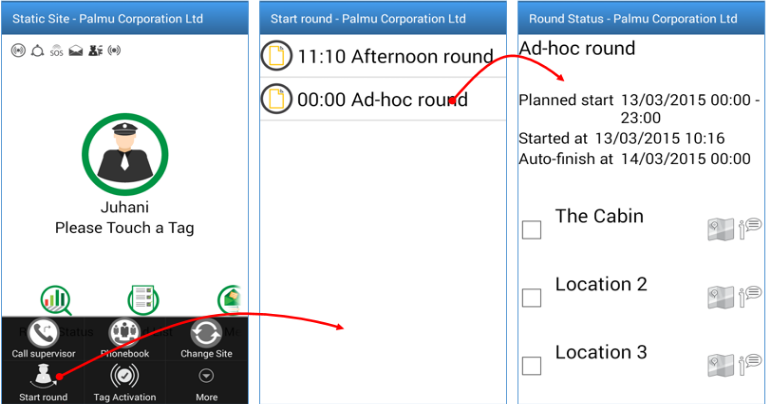
\includegraphics[width=0.9\textwidth]{images/start_round.png}
			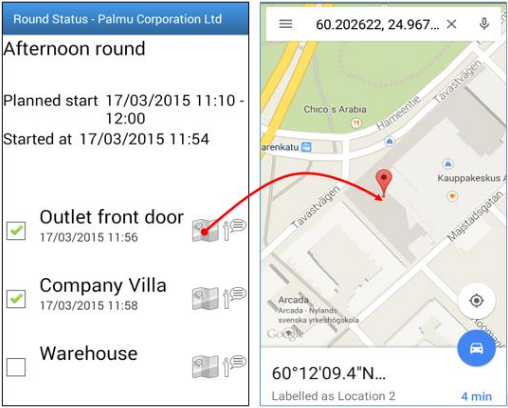
\includegraphics[width=0.6\textwidth]{images/round_status.png}
			\caption{Round planning on the employees' mobile phone.}
			\label{round_on_mobile}
		\end{center}
	\end{figure}
	
	Managers can retrieve real time and historical data about the rounds through the round reports. The round reports module can list the ongoing rounds at one particular moment as well as visualize them on the map and charts as they are being executed. 
	
	At the checkpoints, guards might have to perform some maintenance or some location-specific tasks. For instance, checking if all windows are closed, there is no sign of disturbance. This is possible by presenting short forms on the device, which guards are asked to fill in at certain locations. The mobile phones have the capability to record textual or media data (pictures or video), which can be reported as an incident. 
	
	% offline mode
	Weak internet connection or disruption in the service is not a problem. The Reslink applications are fully functional in offline mode. The loss of internet connection is completely seamless to employees and the generated data is sent as soon as the device finds stable internet connection. 
	
	% alarms
	Alarms can be defined in the back-office. This means that certain transactions generated by the mobile clients are monitored upon they are registered in the central database. In such case, managers are notified immediately by e-mail or text message, so they can take immediate action to resolve the incident. Alarms can be customized to include data concerning where the incident has happened, what the GIS coordinates of the device are, who is the employee reporting the incident and so on. Furthermore, in the back-office supervisors can visualize historical data about alarms on the dashboards. This provides business-critical information such as the reasons and tendencies behind the incidents can be identified by analysts. 
	
	\begin{figure}[h] 
		\begin{center}
		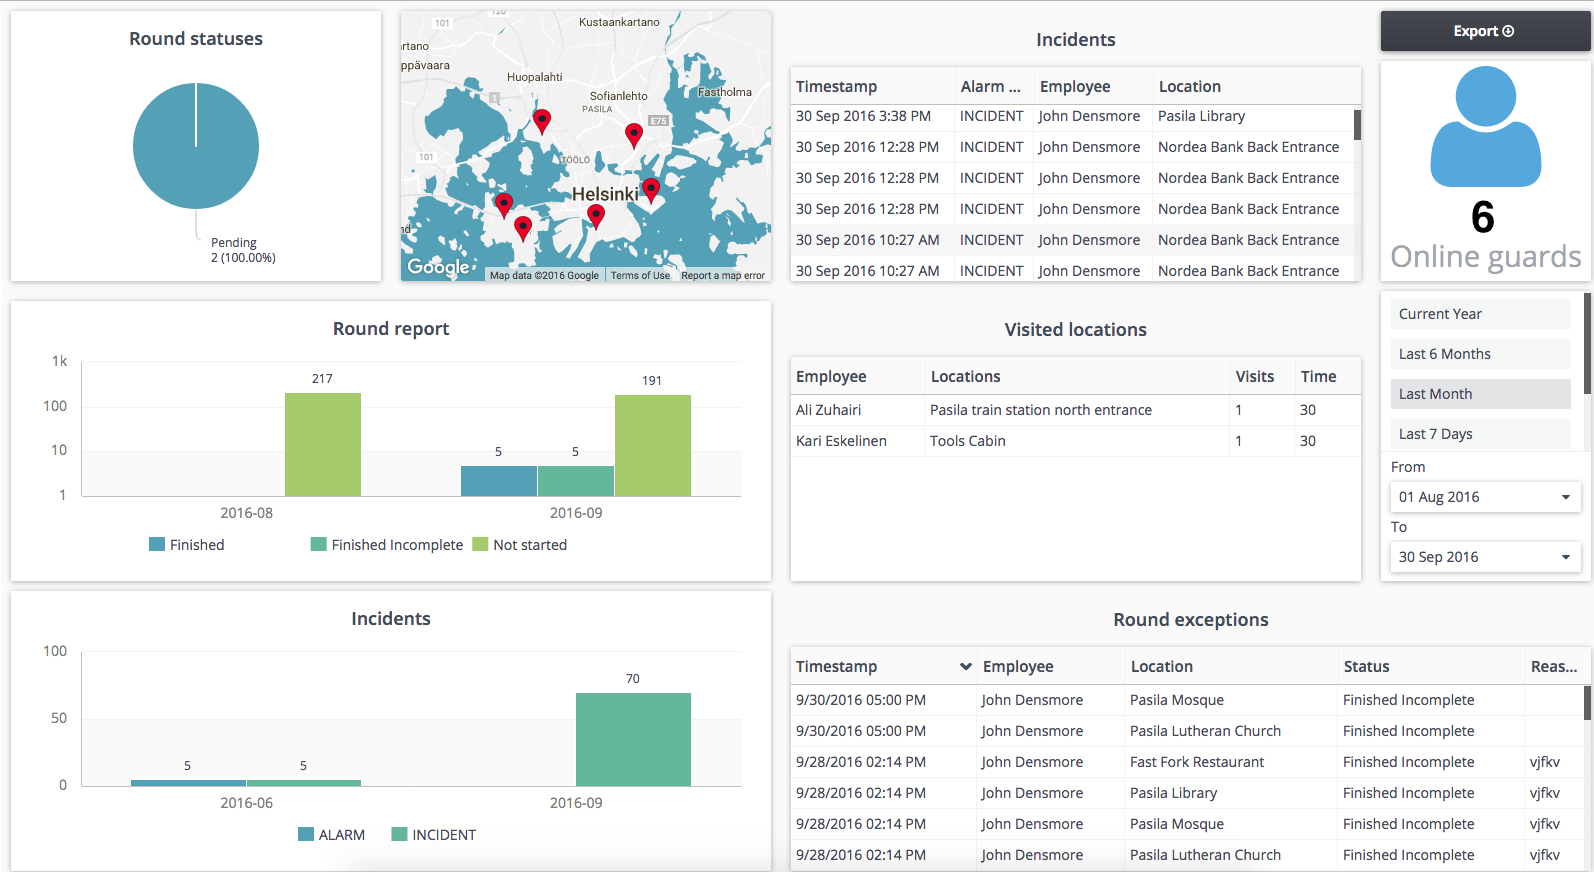
\includegraphics[width=\textwidth]{images/security_dashboard.png}
		\caption{Security dashboard}
		\label{security_dashboard}
		\end{center}
	\end{figure}
	
	Rounds and incidents can be supervised in the back-office on similar dashboards as displayed on Figure \ref{security_dashboard}. The dashboard designed specifically for security industry displays the current statuses of ongoing rounds, the map of employees, the list of incidents, the number of online guards, the historical round report, the visited locations, the incidents' history and the list of round exceptions on one screen. 
	
	Using the dashboards and automated reports supervisors can always ensure that the surveillance of incidents is up and running. As an extension to that, the real-time e-mail and text message notifications provide prompt updates when something unexpected happens on the field. Using the interactive filters supervisors can drill in and see data specifically for locations, employees, areas or time-frames. The automated reporting module has the capability to schedule the report generation, for instance at the end of every month, quarter or year.
	
	The customers of Reslink benefit tremendously from the platform's capabilities. The tools and practices above provide great overview on the key metrics, exceptions and what is happening on the field. Scheduling the rounds and configuring alarms allows supervisors to ensure safety of the facilities at all time. Employees can perform most of their job using one device that can store valuable information, which was not available previously. By utilizing mobile solutions, guards can get from checkpoint to checkpoint quickly and perform the administrative tasks more efficiently.
	
	One of the limitations of the Reslink platform is the employee-time scheduling. Currently, the platform has the capability to answer only the following questions: 
	\pagebreak
	\begin{itemize}
		\item which checkpoints are included in a round?
		\item when the round is executed?
		\item what was the lifecycle of the round during the execution?
		\item who performed this round and when?
	\end{itemize}	 
	In many cases supervisors would like to plan their resources in advance. In this context that would mean assigning employees to rounds and "booking" time in their calendar in advance. This kind of proactive planning would give great values to supervisors, because they could plan their resources in advance. The current solutions are limited to controlling and retrospective and exclude many possibilities for planning and forecasting.
	
\section{Conclusions}
	The advent of smart mobile devices created a lot of possibilities to enhance our productivity. All of a sudden mobile phones were used not only for communication but planning activities, navigating from one place to another and even performing work-related tasks. Realizing the limitless capabilities, many companies started to utilize these devices for performing work-related activities.
	
	The technological possibilities enable firms to optimize traditional processes through smart devices. The continuous Internet connection allows reporting and handling data from mobile phones in real time. Therefore, the paper based administration is fading into the past and being replaced by digital forms filled on mobile devices. On top of that, devices can perform complex calculations reliably, collect precise location and audiovisual data easily. Numerous companies utilize mobile solutions for workforce management in different business fields including guarding, home care, cleaning and technical maintenance. As a result, the concept of mobile workforce was born. 
	
	In this study, a research on the concept of mobile workforce was done. The possibilities, challenges and application fields of utilizing mobile solutions for workforce management were discussed. It was identified that the employees and managers are the main stakeholders in such ecosystem and expect different values from the system. Employees would like to get the benefits for performing their everyday work-related activities, while managers would like to have track on the KPIs and the events happening on the field.
	
	As a single case study, some part of the Reslink platform was introduced. It was demonstrated what tools the company uses to efficiently serve the needs of the guarding industry. The platform offers dashboards and automated reports that facilitate everyday work of supervisors and managers. The former displays the most important KPIs and allows monitoring the events happening on the field, while the latter notifies managers if something unexpected happens on the field. As soon as something unexpected or crucial happens, managers are notified by text message or e-mail, which allows them to take immediate action. The presented case study offers groundbreaking solutions across multiple industries and nations. 
	
	Potential future work could include an in-depth analysis of the mobile workforce management systems on the current market. The Reslink platform could be further analyzed to identify potential bottlenecks and improvement possibilities. It would be interesting to see other case studies how mobility is utilized and how mobile data is represented in different business fields than guarding industry. 
	
\pagebreak

\nocite{*}

\bibliographystyle{tktl}
\bibliography{bibliorgaphy}

\lastpage
\appendices
\pagestyle{empty}
\end{document}


